\documentclass[a4paper, 12pt]{report}
\usepackage{graphicx}
\usepackage{fancyhdr}
\usepackage{wrapfig}
\pagestyle{fancy}
\begin{document}

\graphicspath{{./images/}}
\title{Smarter and simple Scrabble strategy}
\date{Course: DD143X \\ Supervisor: Johan Boye \\ Kungliga Tekniska Högskolan \\ CSC \\ March 7, 2012}
\author{Frej Connolly \\ Götgatan 78 13TR LÄG1302 \\ 118 30 Stockholm \\ SWEDEN \\ +46(0)73-963 41 90 \\ connolly@kth.se \\
        \and Diana Gren \\ Sköldgatan 8 2TR \\ 118 63 Stockholm \\ SWEDEN \\ +46(0)70-467 47 20 \\ dianagr@kth.se}

\maketitle
\begin{abstract}
The abstract goes here.
\end{abstract}
\tableofcontents


\chapter{Results}
\section{Swedish dictionary}
The longest word in the used dictionary is ammoniumdiamintetrakistiocyanatokromat. The shortest possible word to place on board is all two letter words Section \ref{regler}. The number of two letter words is 121. Table \ref{table:dictionary+length}.
\begin{table}[h]
\centering
	\begin{tabular}{l | c | c}
	& Base words & All words \\
	\hline
	Mean & 9.5 & 11.2 \\
	\hline
	Longest & \multicolumn{2}{c}{ammoniumdiamintetrakistiocyanatokromat} \\
	\hline
	Shortest & \multicolumn{2}{c}{121 two letter words} \\ 
	\end{tabular}
\caption{Mean, largest and smallest lengths of legal words in the dictionary.}
\label{table:dictionary+length}
\end{table}

\section{Bonus squares vs High score words}
\emph{BS} wins just over 6 of 10 times against \emph{HSW} when using all inflection forms from the Swedish dictionary table \ref{table:bs+hsw+allwords} and well over 5 of 10 times when only the base forms of words is used table \ref{table:bs+hsw+baseforms}. When \emph{BS} started playing it won 52\% of its wins when using all inflection forms. For \emph{HSW} 53\% of its wins. When using only the base form both of them were winning 51\% its wins when started laying out words.

The resulting mean, median, highest and lowest scores is significant higher when using all inflection forms. Lowest score is negative for both players when using only base forms. \emph{BS} mean score is 24\% higher in table \ref{table:bs+hsw+allwords} compared to table \ref{table:bs+hsw+baseforms}. The same applies for the end score which is higher when using all words Appendix Figure \ref{fig:bs+hsw+totalscores}.

\begin{table}[h]
\centering
    \begin{tabular}{ l | l | l }
   	& Bonus Squares & High score words \\
   	\hline
   	Wins & 6104 & 3857 \\
	Wins when started playing & 3148 & 2040 \\   	
	Mean score & 308 & 278 \\
	Median score & 301 & 273 \\	 	 
	Highest score & 724 & 606 \\
	Lowest score & 85 & 61 \\		
	\hline 
   	Draws & 39 & 39 \\
    \end{tabular}
\caption{Result from 10 000 games with words in all inflection forms from the Swedish dictionary (480 391 words).}
\label{table:bs+hsw+allwords}
\end{table}

\begin{table}[h]
\centering
    \begin{tabular}{ l | l | l }
   	& Bonus Squares & High score words \\
   	\hline
   	Wins & 5427 & 4521 \\
	Wins when started playing & 2758 & 2314 \\   	
	Mean score & 248 & 240 \\
	Median score & 246 & 234 \\	 	 
	Highest score & 488 & 506 \\
	Lowest score & -15 & -11 \\		
	\hline 
   	Draws & 52 & 52 \\
    \end{tabular}
\caption{Result from 10 000 games with only words in base form from the Swedish dictionary (83 247 words).}
\label{table:bs+hsw+baseforms}
\end{table}


\chapter{Conclusions}
\subsubsection{BS player}
Choosing to place words that will occupy a bonus square is rewarding. It will not only give a high score but will also destroy the possiblity for the opponent to reach a bonus square.

It has active playing style with the mission to conquer the bonus squares at all cost. With the power of a big dictionary it will have a higher probability to reach a bonus. It is easy to extend words already on board when having the possibility to use all inflection forms of words. The end score will also be higher Figure \ref{fig:bs+hsw+totalscores}. When using only base words it will struggle to find bonus squares. This is due to 


\subsubsection{HSW player}
The 

\chapter{appendix}
\begin{figure}[h]
\centering
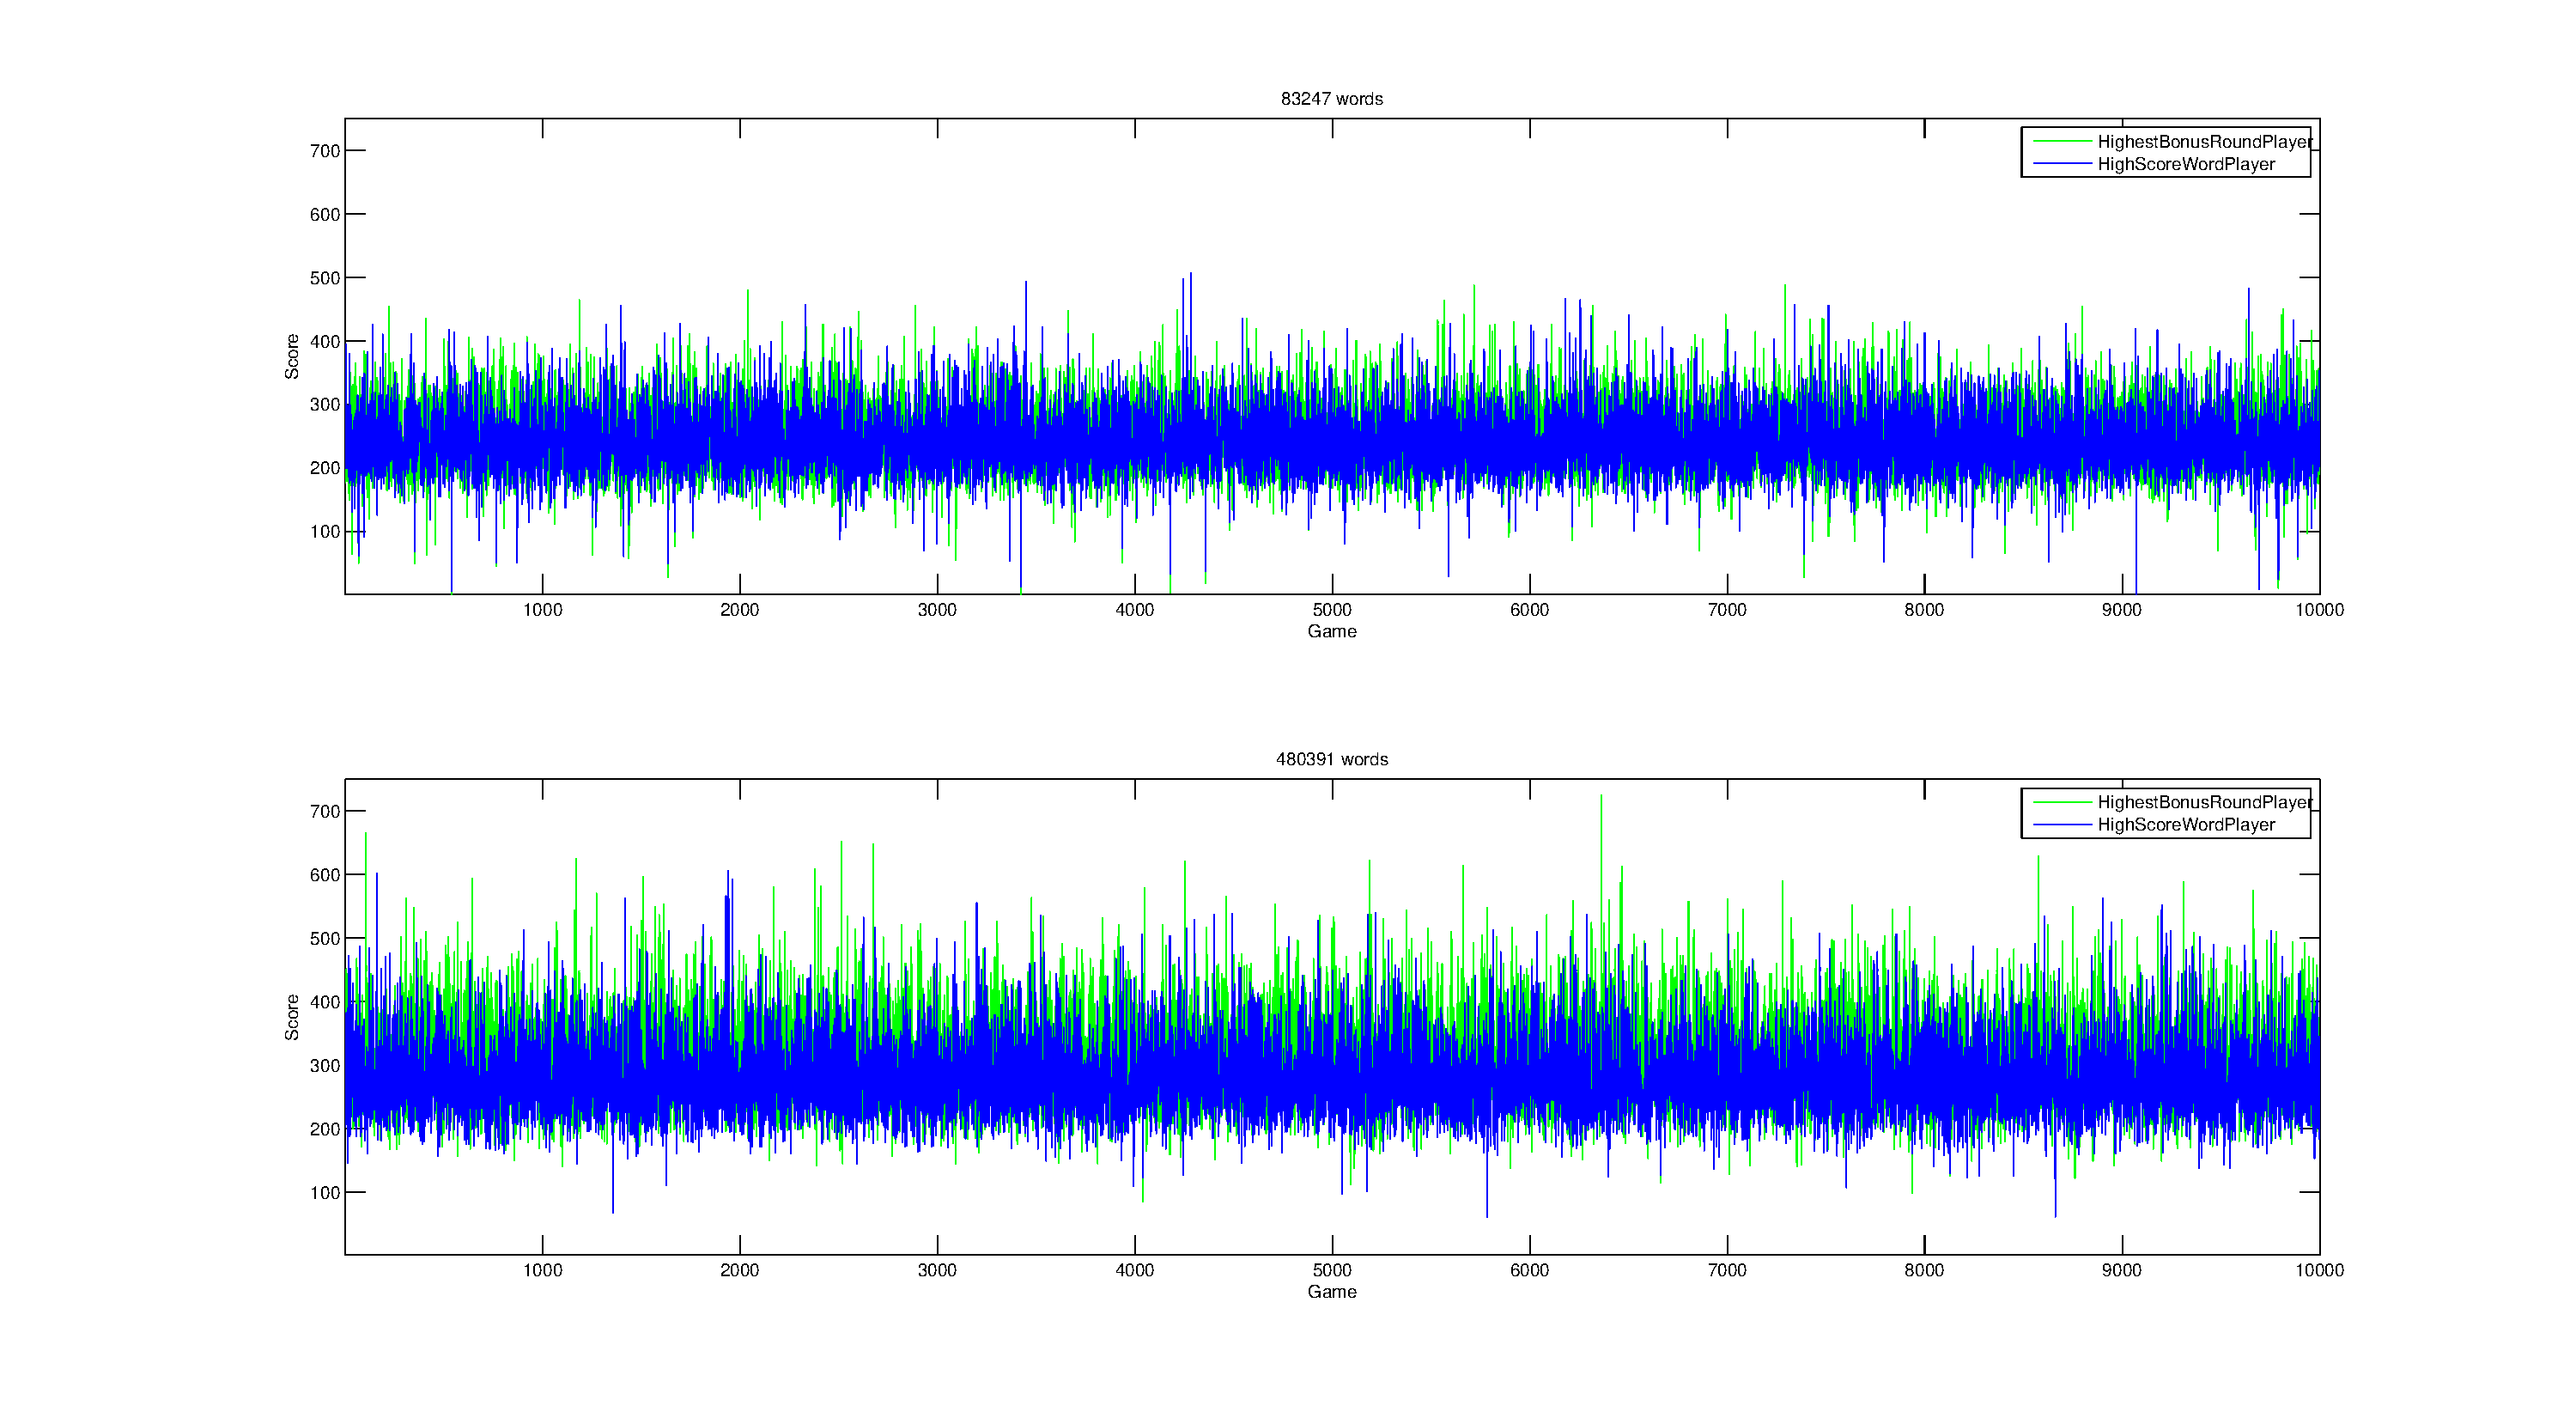
\includegraphics[scale=0.3]{Highest_Bonus_Round_vs_High_Score_Word_10000}
\caption {End scores of the two players in 10000 games. Upper graph with base words only and lower graph with all inflection forms.}
\label{fig:bs+hsw+totalscores}
\end{figure}

\begin{thebibliography}{100}  
\bibitem{dictionary}Den stora svenska ordlistan, %http://code.google.com/p/dsso/downloads/detail?name=dsso-1.52.txt&can=1&q=
\end{thebibliography}
\end{document}